\section{Cavity QED}
Let us consider an atom inside an optical cavity. The EM field modes in the cavity correspond 
to standing wave modes with a frequency spacing $\Delta\omega=\pi c/L$ between adjacent modes.
\begin{figure}[htbp]
    \centering
    \begin{subfigure}{.45\columnwidth}
        \centering
        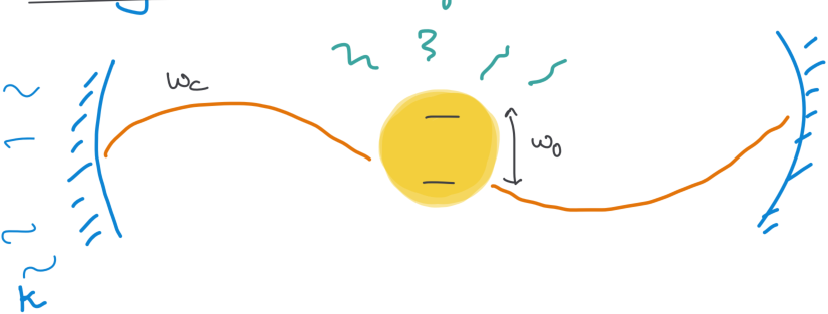
\includegraphics[width=\columnwidth]{PartOne/ChapterFour/figures/cavityqed_1.png}
        \caption{Cavity}
    \end{subfigure}
    \hfill
    \begin{subfigure}{.4\columnwidth}
        \centering
        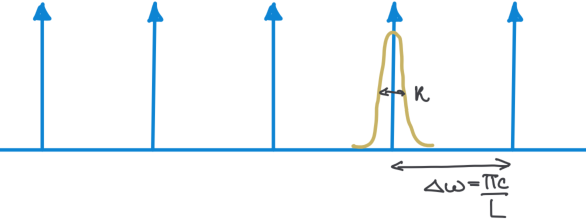
\includegraphics[width=\columnwidth]{PartOne/ChapterFour/figures/cavityqed_2.png}
        \caption{Modes spectrum}
    \end{subfigure}
    \caption{Cacity QED and modes.}
\end{figure}

In the presence of lossy mirrors the cavity has a decay such that there is a Lorentzian linewidth $\kappa$ to each 
cavity resonance. 

Consider a cavity of length $L\ll\lambda_0$, the fundamental mode of the cavity starts at 
\begin{align}
    \underbrace{\omega_{c0}=\frac{\pi c}{L}}_{\text{cavity fundamental mode}}\gg\underbrace{\omega_0=\frac{\pi c}{\lambda_0}}_{\text{Atomic resonance}}.
\end{align}
To such a case the atom does not see any modes to emit into and its spontaneous emission is inhibited.
More generally cavity modifies the EM field mode structure seen by the atom. A typical Fabry-Perot cavity is 
$\sim100\;\mu m$ long with $\Delta\omega\sim10^{13}\;Hz$.

In such a regime the atom typically only sees one of the modes of the EM field inside the cavity. 
The total atom+cavity system is described by the Hamiltonian:
\begin{align*}
    H=H_A+H_C+H_{AC},\quad\begin{array}{l}
        H_A=\hbar\omega_0\hsigma_+\hsigma_-\\
        H_C=\hbar\omega_c\ha^\dagger\ha\\
        H_{AC}=-\hbd\cdot\hbE(\br_A)=-(\bd\hsigma_++\bd^*\hsigma_-)\cdot\sqrt{\frac{\hbar\omega_c}{2\varepsilon_0V}}\he_c(\ha+\ha^\dagger)\sin(k_cr_a).
    \end{array}
\end{align*}
Making RWA, we have 
\begin{align*}
    H_{AC}=\underbrace{-\bd\cdot\he_c\sqrt{\frac{\hbar\omega_c}{2\varepsilon_0V}}\sin(k_cr_a)}_{i\hbar g}[\hsigma_+\ha+\hsigma_x\ha^\dagger].
\end{align*}
The total Hamiltonian is therefore:
\begin{align}
    \text{Joynes-Cumming Hamiltonian}\qquad H=\hbar\omega_0\hsigma_+\hsigma_-+\hbar\omega_c\ha^\dagger\ha+i\hbar g[\hsigma_+\ha+\hsigma_x\ha^\dagger].
\end{align}
The above Hamiltonian conserves the total number of excitations such that the eigenstates of the Hamiltonian can be expressed 
in terms of linea combinartions of $\{\ket{g,n},\ket{e,n-1}\}$ in the n-excitation manifold.
\begin{align*}
    \ket{\Psi_n}=c_{gn}\ket{g,n}+c_{e,n-1}\ket{e,n-1}.
\end{align*}
From Schrodinger equation:
\begin{align*}
    i\hbar\partial_t\ket{\Psi_n}&=H\ket{\Psi_n}\\
    \partial_t\begin{bmatrix}
        c_{e,n-1}\\c_{g,n}
    \end{bmatrix}&=-\frac{i}{\hbar}\begin{bmatrix}
        (n-1)\hbar\omega_c+\hbar\omega_0&i\hbar g\sqrt{n}\\
        -i\hbar g\sqrt{n}&n\hbar\omega_c
    \end{bmatrix}
    \begin{bmatrix}
        c_{e,n-1}\\c_{g,n}
    \end{bmatrix}.
\end{align*}
From diagonalizing the Hamiltonian in the n-ecitation manifold the eigenstates of the atom+field system are:
\begin{align*}
    \ket{+,n}&=i\sin\theta_n\ket{g,n}+\cos\theta_n\ket{e,n-1}\\
    \ket{-,n}&=-\cos\theta_n\ket{g,n}+\sin\theta_n\ket{e,n-1},\quad\tan2\theta_n=\frac{2g\sqrt{n}}{\Delta_c},\;\Delta_c=\underbrace{\omega_0-\omega_c}_{\text{cavity detuning}}.
\end{align*}
The eigenenergies are:
\begin{align*}
    E_n^\pm=\frac{\hbar}{2}\left[\omega_0+(2n-1)\omega_c\pm\sqrt{4g^2n+(\omega_0-\omega_c)^2}\right].
\end{align*}

\begin{itemize}
    \item\text{Uncoupled case $g\to0$} 
    \begin{align*}
        E_n^\pm&=\frac{\hbar}{2}[\omega_0+(2n-1)\omega_c\pm(\omega_0-\omega_c)]\\
        \ket{e,n-1}:\;E_n^+&=\frac{\hbar}{2}[2\omega_0+2(n-1)\omega_c]=\hbar(\omega_0+(n-1)\omega_c)\\
        \ket{g,n}:\;E_n^-&=\frac{\hbar}{2}[2n\omega_c]=\hbar n\omega_c.
    \end{align*}
    \item\textbf{Resonant case $\Delta_c\to0$}
    \begin{align*}
        E_n^\pm=\frac{\hbar}{2}[\omega_0+(2n-1)\omega_c\pm2h\sqrt{n}]=n\hbar\omega_c\pm\hbar g\sqrt{n}.
    \end{align*}
    Eigenstates are:
    \begin{align*}
        \ket{+,n}&=\frac{1}{\sqrt{2}}[i\ket{g,n}+\ket{e,n-1}]\\
        \ket{-,n}&=\frac{1}{\sqrt{2}}[-i\ket{g,n}+\ket{e,n-1}]
    \end{align*}
\end{itemize}

\textbf{Example}: How does an excited atom evolve in an empty resonant single-mode cavity?
The initial state of the system $\ket{e,0}$.
\begin{align*}
    \text{states in the single subspace}\quad\ket{e,0}\to\ket{g,1}.
\end{align*}
The eigenstates are:
\begin{align*}
    \ket{+,1}&=\frac{1}{\sqrt{2}}[i\ket{g,1}+\ket{e,0}],\;E_+=n\hbar\omega_c+\hbar g\\
    \ket{-,1}&=\frac{1}{\sqrt{2}}[-i\ket{g,1}+\ket{e,0}],\;E_-=\hbar\omega_c-\hbar g.
\end{align*}
The initial state can be written in terms of the eigenstates as:
\begin{align*}
    \ket{e,0}&=\frac{1}{\sqrt{2}}[\ket{+,1}+\ket{-,1}]\\
    &\text{each eigenstate evolves with the corresponding eigenenergies}\\
    &\frac{1}{\sqrt{2}}[\ket{+,1}e^{-iE_+t/\hbar}+\ket{-,1}e^{-iE_-t/\hbar}]\\
    &=\frac{1}{2}[\{i\ket{g,1}+\ket{e,0}\}e^{-i\omega_ct}e^{-igt}+\{-i\ket{g,1}+\ket{e,0}\}e^{-i\omega_ct}e^{igt}]\\
    &=\frac{1}{2}e^{-i\omega_ct}[i\ket{g,1}\{e^{-igt}-e^{igt}\}+\ket{e,0}\{e^{igt}+e^{-igt}\}]\\
    &=e^{-i\omega_ct}[\sin(gt)\ket{g,1}+\cos(gt)\ket{e,0}].
\end{align*}
Vacuum Rabi oscilattions of an atom in a single mode cavity.
\begin{figure}[htbp]
    \centering
    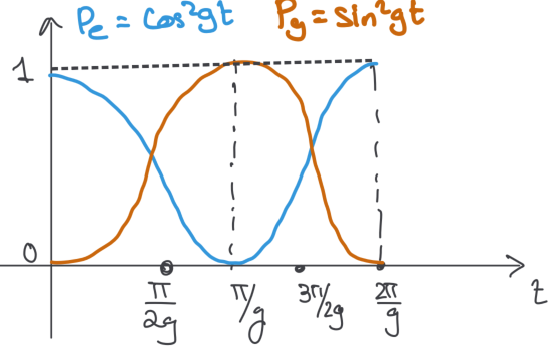
\includegraphics[width=.5\columnwidth]{PartOne/ChapterFour/figures/cavityqed_rabi}
    \caption{Rabi oscilaltion in a single-mode cavity.}
\end{figure}